\subsection{Safety Assessment Process}
\label{subsec:process}

ARP4754A, the Guidelines for Development of Civil Aircraft and Systems~\cite{SAE:ARP4754A}, has been recognized by the Federal Aviation Administration (FAA) as an ``acceptable method for establishing a development assurance process''~\cite{AC:20-174}. It provides guidance on applying development assurance at each hierarchical level throughout the development life cycle of highly-integrated/complex aircraft systems.

%Figure~\ref{fig:arp4754a_process} from [ref. ARP4754A] demonstrates the ARP4754A process flow.

The safety assessment process is a starting point at each hierarchical level of the development life cycle, and is tightly coupled with the system development and verification processes. It is used to show compliance with certification requirements, and meeting a company's internal safety standards~\cite{SAE:ARP4754A}. ARP4761, the Guidelines and Methods for Conducting Safety Assessment Process on Civil Airborne Systems and Equipment~\cite{SAE:ARP4761},  identifies a systematic means to show compliance. The guidelines presented in ARP4761 include industry accepted safety assessment processes (Functional Hazard Assessment (FHA), Preliminary System Safety Assessment (PSSA), and System Safety Assessment (SSA)), and safety analysis methods to conduct the safety assessment, 
such as Fault Tree Analysis (FTA), Failure Modes and Effect Analysis (FMEA), and Common Cause Analysis (CCA).

\iffalse
\begin{figure}[h!]
	\vspace{-0.19in}
	\begin{center}
		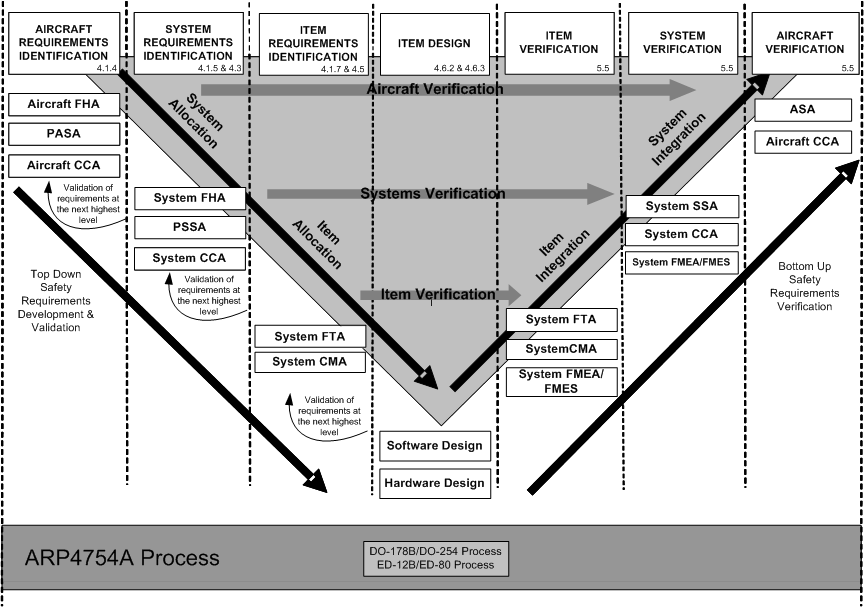
\includegraphics[trim=0 9 0 5,clip,width=1.0\textwidth]{images/ARP4754A_Process.png}
	\end{center}
	%\vspace{0.4in}
	\caption{ARP4754A Process(from ARP4754A ref)}
	\label{fig:arp4754a_process}
\end{figure}
\fi

A prerequisite of performing the safety assessment of a system design is to understand how the system works, primarily focusing on the integrity of the outputs and the availability of the product. The safety engineers then use the acquired understanding to construct the safety analysis artifacts, conduct safety analysis, and compare the analysis results with established safety objectives and safety related requirements.

In practice, prior to performing the safety assessment of a system, the safety engineers are often equipped with fair amount of knowledge on how system works in general, but not necessarily with the specific system \mike{I don't know what the previous sentence means...do you mean 'in principle?' rather than 'in general'}. \janet{It was meant to say that they know at a high level how system like this should work and the safety pitfalls, but not the detailed information about the specific system} Acquiring the knowledge on the content and behavior of a specific system has shown to be time consuming to get it right. In one real case example, it took a safety engineer two full working days to understand how the software works in a Stall Warning System (a dual channel system involving six main system-level functions such as input signal processing) \mike{'solid' might be overkill}.  \mike{this needs a little bit of wordsmithing} \janet{changed 'two solid days' to 'two full working days'} The primary task includes connecting the signal and function flows to relate the input and output signals from end-to-end and understanding the causal effect between them. This is the same amount of time, if not more, as constructing the analysis artifacts and performing the analysis itself. In another real case example, it took a safety engineer almost a year to finalize the PSSA document for a Horizontal Stabilizer Control System (a dual channel dual lane system involving eighteen main system-level functions and clean-sheet design), involving two major revisions and multiple rounds of reviews with system, hardware, and software engineers.

Capturing failure mode in models and generating safety analysis artifacts directly from models can enhance communication and synchronization between system design process and safety assessment process, and the ability to analyze complex systems. Industry practitioners have come to realize the benefits and importance of
using models to assist the safety assessment process (either by augmenting the existing system design model, or by building a separate safety model), and a revision of the ARP4761 with model based safety analysis appendix is under way.

Using the same system design model to conduct both system design and safety analysis can help reduce the gap in comprehending the system behavior and transferring the knowledge between the design model to the safety analysis model. It maintains a living model that captures the latest state of the system design as the process flows per the system development lifecycle.
%Figure~\ref{fig:arp4754a_process}.
It also allows all participants of the ARP4754A process to be able to communicate and review the system design using the ``single source of truth''.

In order to allow performing system design and safety analysis on the same model, the system design model will need to be augmented to include both the system design information (e.g., system architecture, functional behavior) and safety-relevant information (e.g., failure mode, failure rate), at the same time keeping the two types of information distinguishable yet interactable from each other.

Figure~\ref{fig:proposed_safety_process} \mike{This reference should be sooner or the figure should be later in the paper - also the figure needs larger font size and a little less space between the boxes} \janet{updated the figure and location} presents our proposed use of the shared system design and safety analysis model (to be referred as ``the shared model" in the rest of this section) inside the ARP4754A Safety Assessment Process Model (Figure 7 of~\cite{SAE:ARP4754A}). As seen in the figure, the shared model represents a system development artifact from the ``Development of System Architecture'' and ``Allocation of System Requirements to Item'' activities in the System Development Process, which interacts with the PSSAs and SSAs activities in the Safety Assessment Process. The shared model can serve as a wrapper and interface to capture the information relevant to safety analysis from the system design and implementation.

\begin{figure}[h!]
	\vspace{-0.19in}
	\begin{center}
		\includegraphics[trim=0 9 0 5,clip,width=0.9\textwidth]{images/Safety_Assessment_Process_update.png}
	\end{center}
	%\vspace{0.4in}
	\caption{Using the Shared System/Safety Model in the ARP4754A Safety Assessment Process}
	\label{fig:proposed_safety_process}
\end{figure}

Figure~\ref{fig:interaction_with_FTA} shows an example how the preliminary FTAs and FTAs (artifacts from the PSSA and SSA activities in the Safety Assessment Process) can guide and be updated from the shared model. The next subsection will describe the foundation of the modeling technique in more details.

\begin{figure}[h!]
	\vspace{-0.19in}
	\begin{center}
		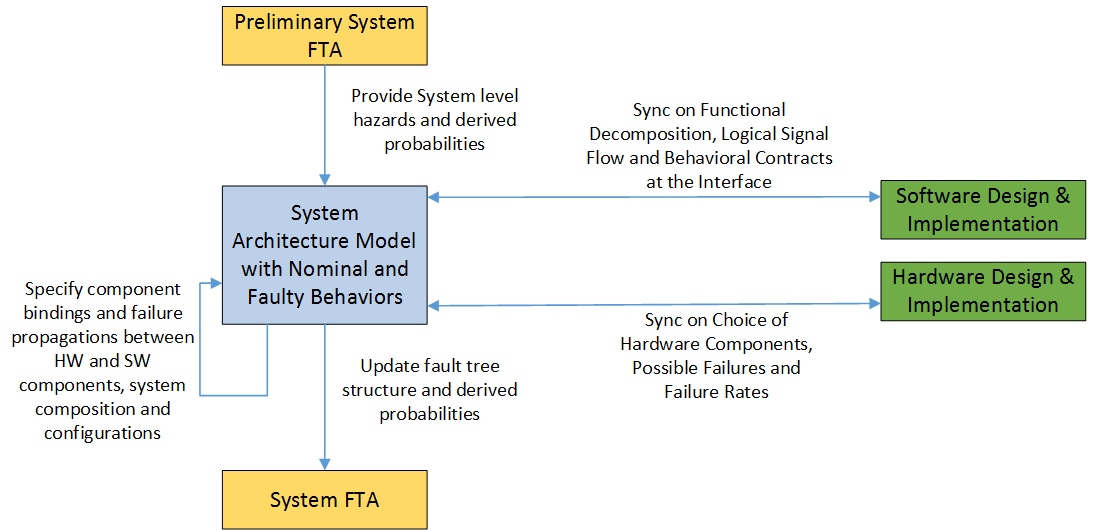
\includegraphics[width=0.9\textwidth]{images/FTA_MBD_Workflow.png}
	\end{center}
	%\vspace{0.4in}
	\caption{Example Interactions between the Shared System/Safety Model and  the FTAs}
	\label{fig:interaction_with_FTA}
\end{figure}
